%!TEX root = ../dissertation.tex

\chapter{Practical Experiments}
\label{chapter:experiments}

The previous sections described the implementation of the tools proposed in Chapter~\ref{chapter:pegd}. This chapter completes the implementation, evaluating these tools with practical experiments, namely using the sketch-program correlation tool to illustrate \gls{gd} programs, and the immediate feedback tool to interactively generate geometric models.

\section{The experiment}

The conducted experiment started by asking a group of architects to install the plugin, in their programming environment. Moreover, to facilitate this process, the source code was placed in a repository publicly accessible. Thus to complete the installation, the users copied the repository URL link into DrRacket Package Manager and the plugin was automatically installed. Once the installation completes, DrRacket was able to load the implemented tools as part of its programming tools. 

It is important to note that the target users that collaborated in this experiment were familiar with \gls{gd} methods. Some of them had already their GD programs documented with sketches. Therefore, to test the capabilities of these tools in real use cases, we suggested them to (1) document a function using a proper sketch, completing the process to associate the function parameters with its illustrated symbols, and (2) explore the immediate feedback tool, using Rosetta tool with an adequate backend, and a parametric model that produces geometry in less than 1 minute.

\section{Program-sketch correlation tool}

Figure~\ref{fig:losa0} shows a \gls{gd} program that has their parameters illustrated in a sketch. In this example, the architect did the design manually, using a piece of paper, then she painted the intended shape using parametric variables to annotate it. Then, the final sketch was scanned, and inserted into the code. Immediately after this process, she moved the mouse over the image and some arrows appeared from the center of the image to the  function parameters.

Figure~\ref{fig:losa1} concludes the prior process showing the result of correcting the associations between the parameters and its symbols. The architect, followed the mechanism explained in Section~\ref{sec:psct} to bind each parameter of the function to a place in the image. Note that, in this example, all arrows are visible because she moved the mouse over to the picture.

Figure~\ref{fig:turbine} shows a program illustrated with three sketches. Unlike the previous example, these sketches were done using a drawing tool. In fact, these images were already included in the program but were not correlated with the code. To use this tool the architect just moved her sketches into the function body, corrected the binding associations, and clicked on Check Syntax button. Therefore, she pointed to a parameter of a function fan-blad and immediately sees its meaning in the image.

\begin{figure}[h]
\centering
\begin{minipage}[t]{.495\textwidth}
  \centering
  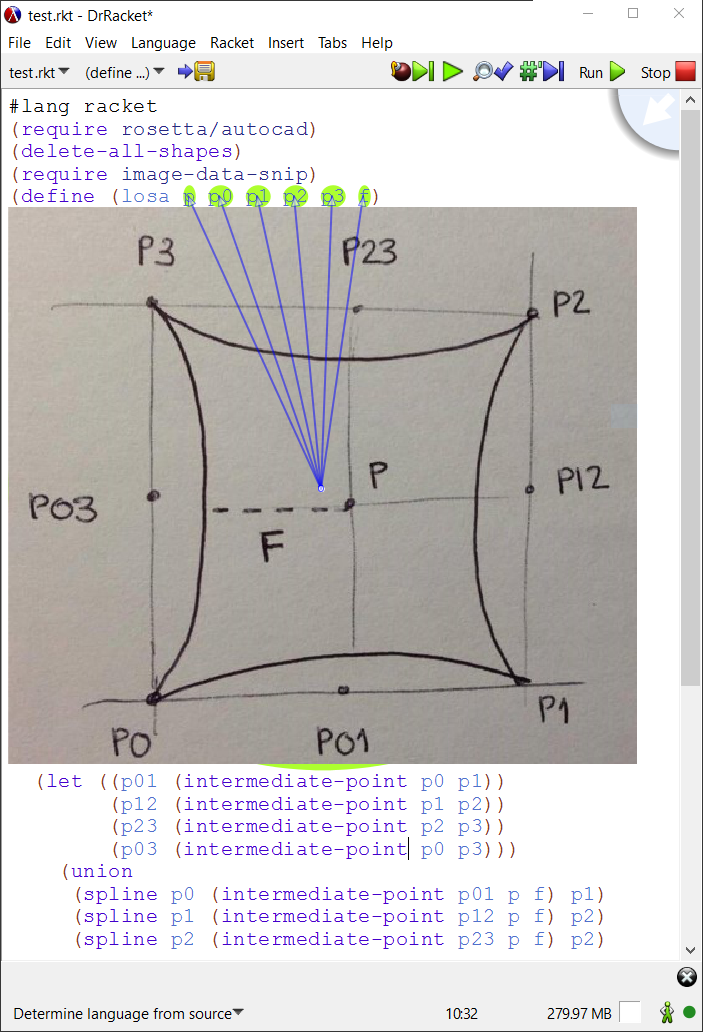
\includegraphics[width=1\linewidth]{images/losa0}
  \captionof{figure}{After inserting a sketch in the function body.}
  \label{fig:losa0}
\end{minipage}%
~
~
\begin{minipage}[t]{.495\textwidth}
  \centering
  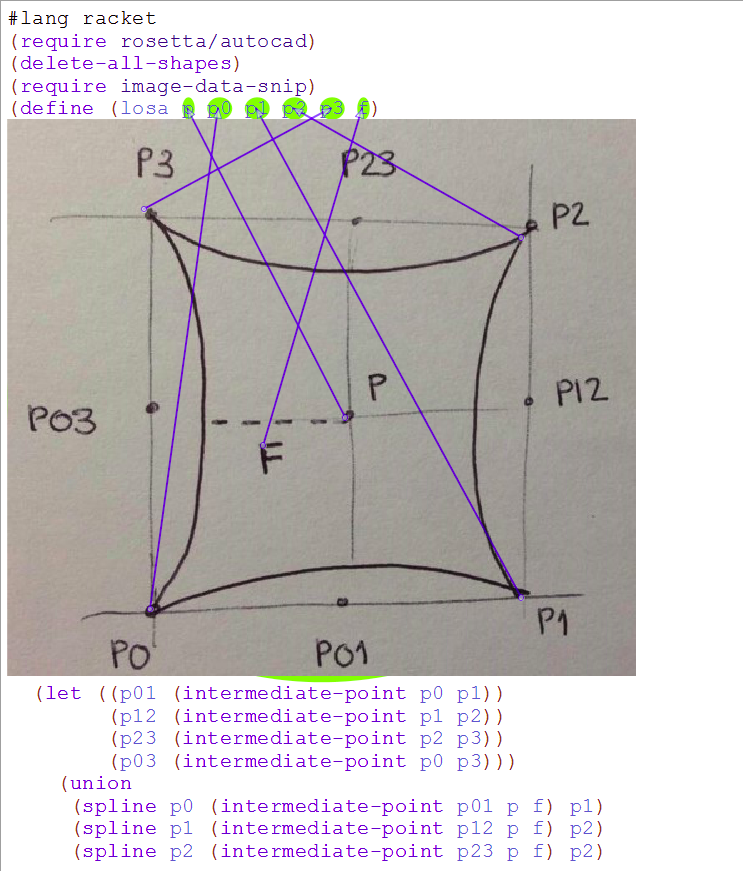
\includegraphics[width=1\linewidth]{images/losa}
  \captionof{figure}{After correcting the associations between the function parameters and its symbols.}
  \label{fig:losa1}
\end{minipage}
\end{figure}

\begin{figure}[!h]
  \centering
  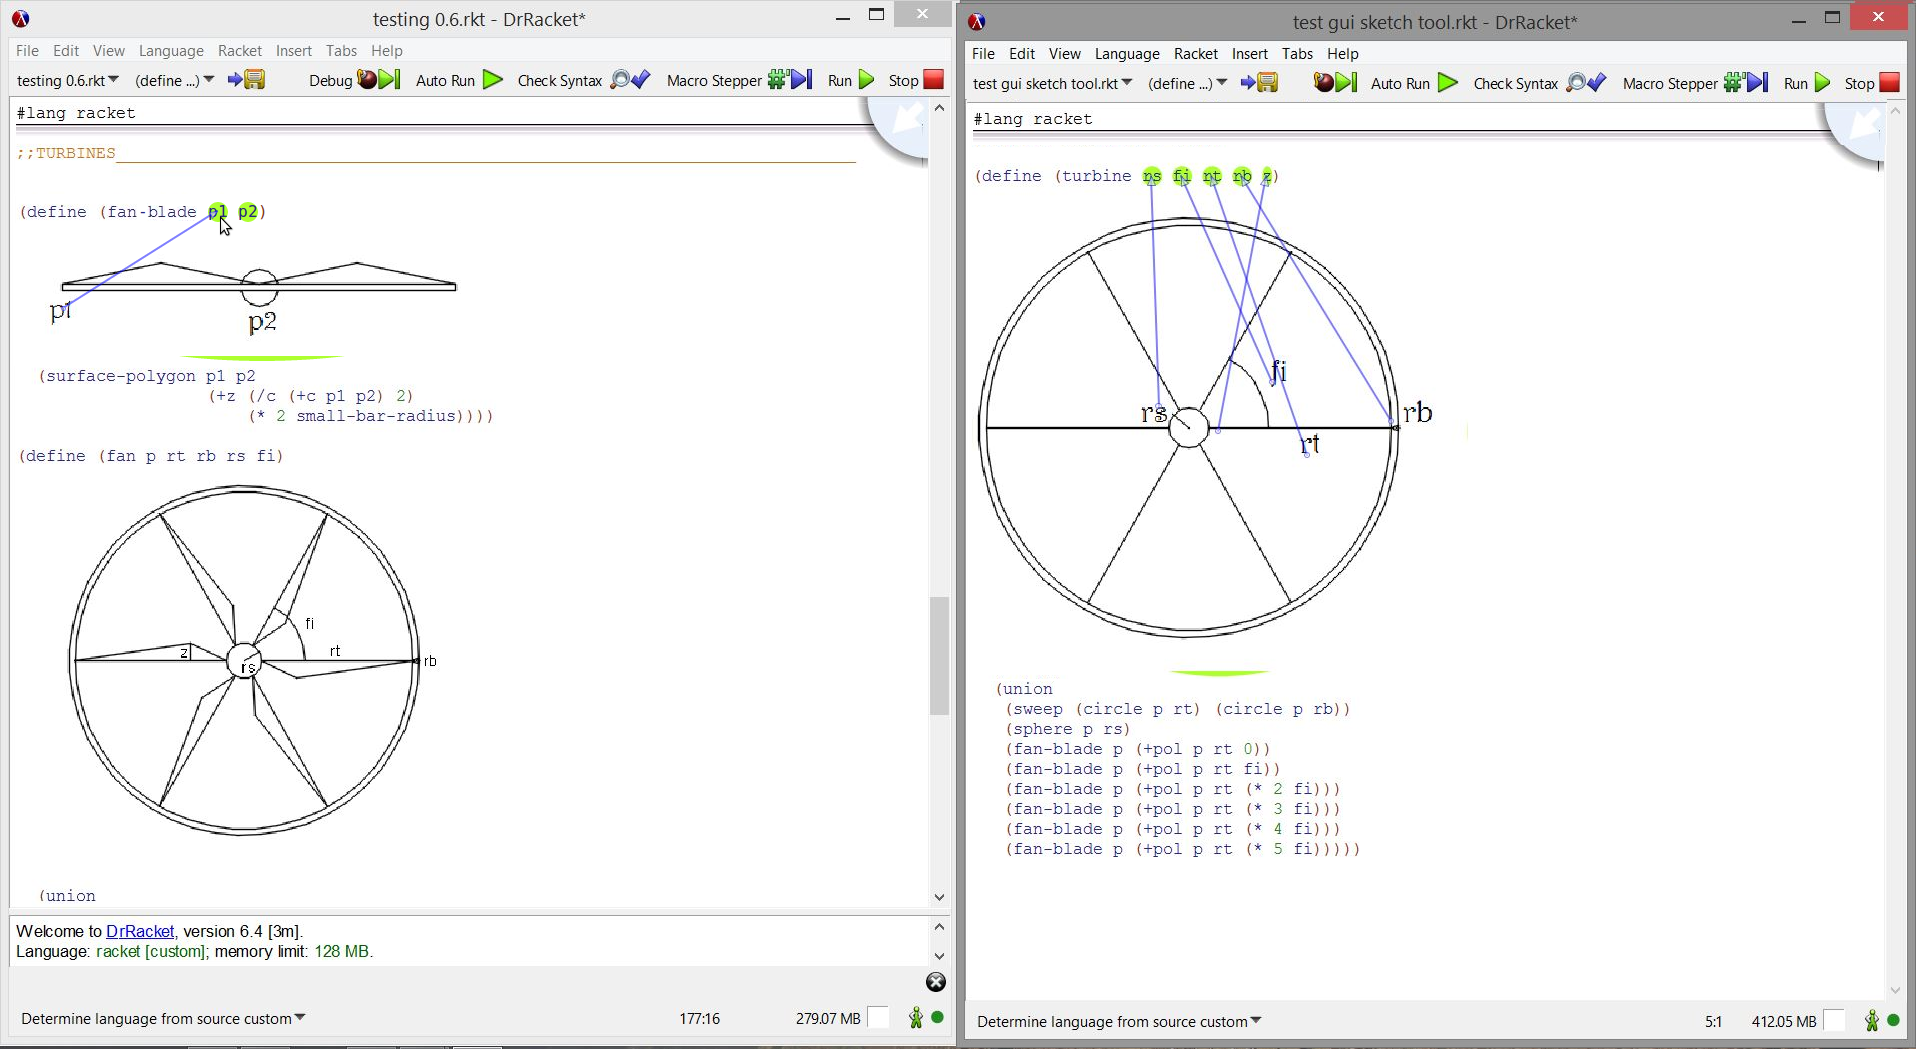
\includegraphics[width=1\textwidth]{images/turbine}
    \caption{Correlating existing sketches with code.}
  \label{fig:turbine}
\end{figure}

\begin{figure}[!h]
  \centering
  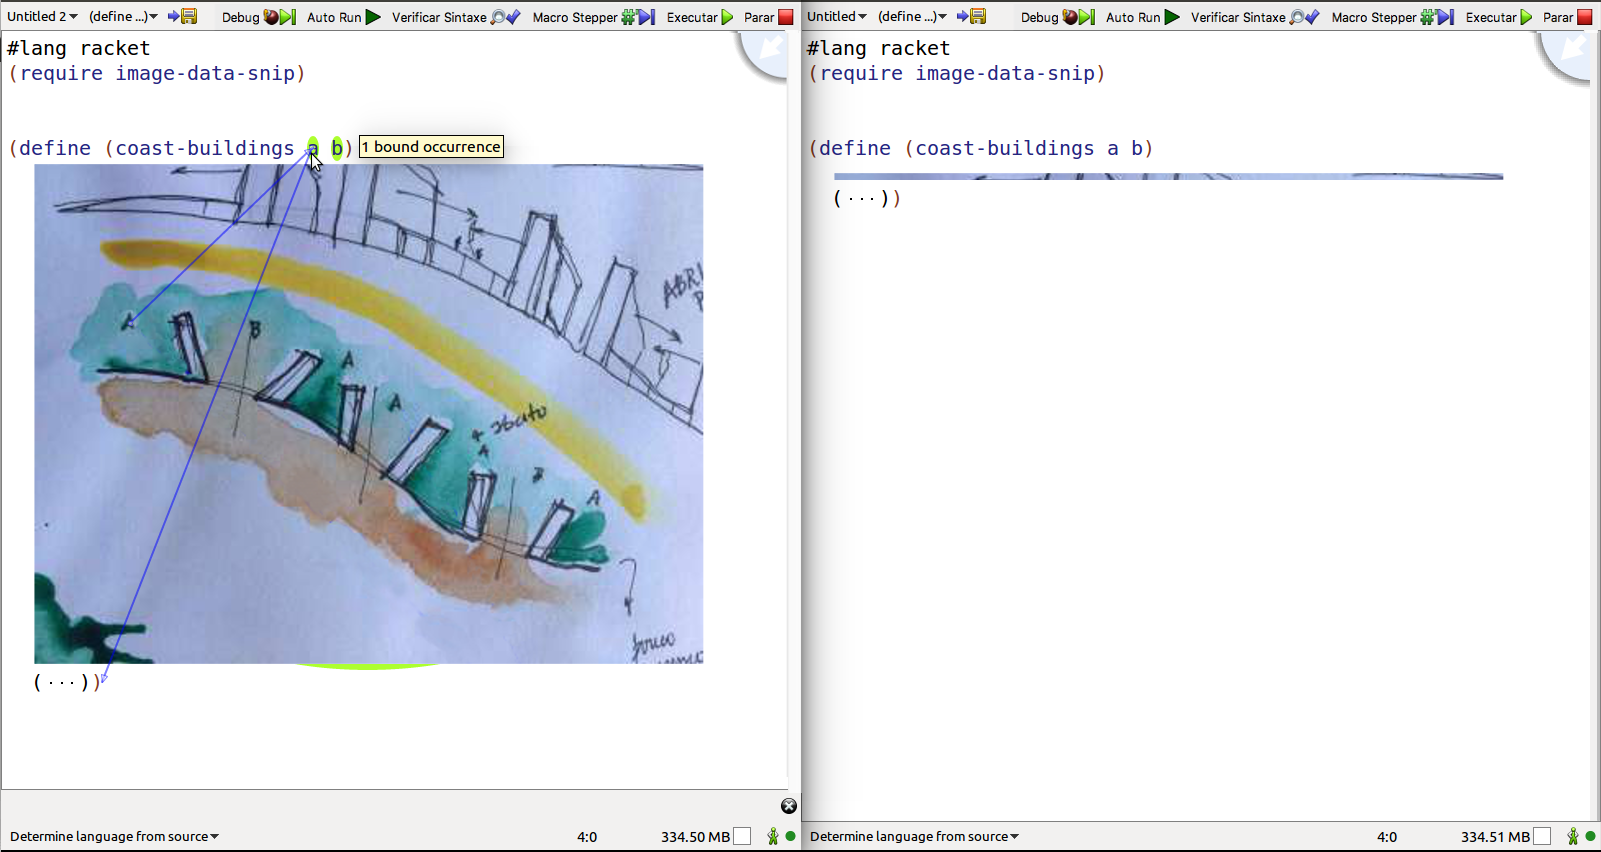
\includegraphics[width=1\textwidth]{images/coast}
    \caption{Collapsing the sketch.}
  \label{fig:coast}
\end{figure}

While the sketches used in the previous examples were intentionally made to illustrate the context of that function, Figure~\ref{fig:coast} shows a sketch in an initial phase of design.  In this example, the architect collapsed the s-expressions and pointed to the parameter \texttt{a}. Then an arrow links the parameter \texttt{a} to the image, and other to the s expression. On the right, the sketch was collapsed reducing the function to a few lines of code.


\section{Immediate feedback tool}

Figure~\ref{fig:s1}, Figure~\ref{fig:s2}, and Figure~\ref{fig:s3} show a sequence of spheres, on the left, rendered by Autocad backend using the function n-spheres, defined on the right. In this example, the architect enabled the active mode in AutoRun plugin and used the slider widget to change the input of n-spheres function.

\begin{figure}[!h]
  \centering
  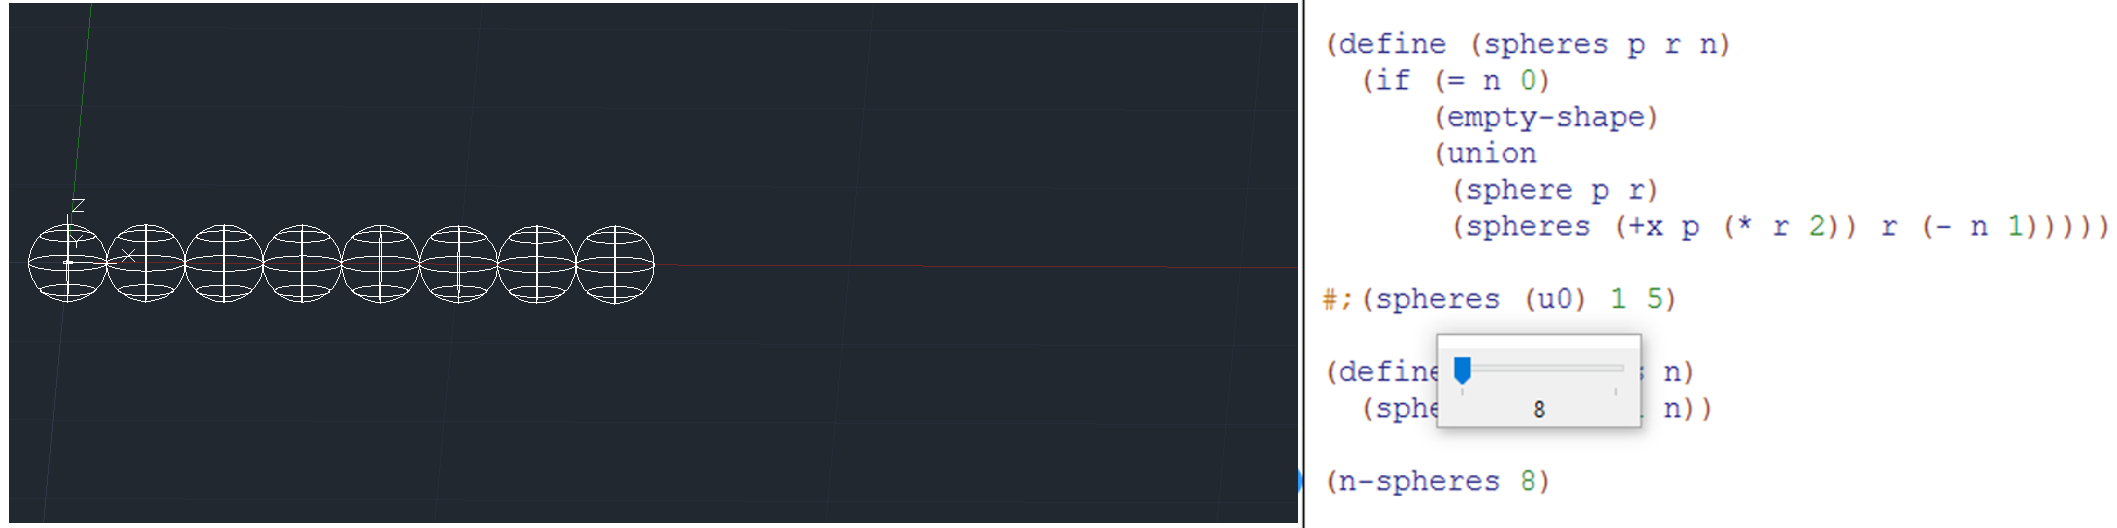
\includegraphics[width=1\textwidth]{images/sliders1}
    \caption{Changing n-spheres input to 8 spheres using a slider.}
  \label{fig:s1}
\end{figure}

\begin{figure}[!h]
  \centering
  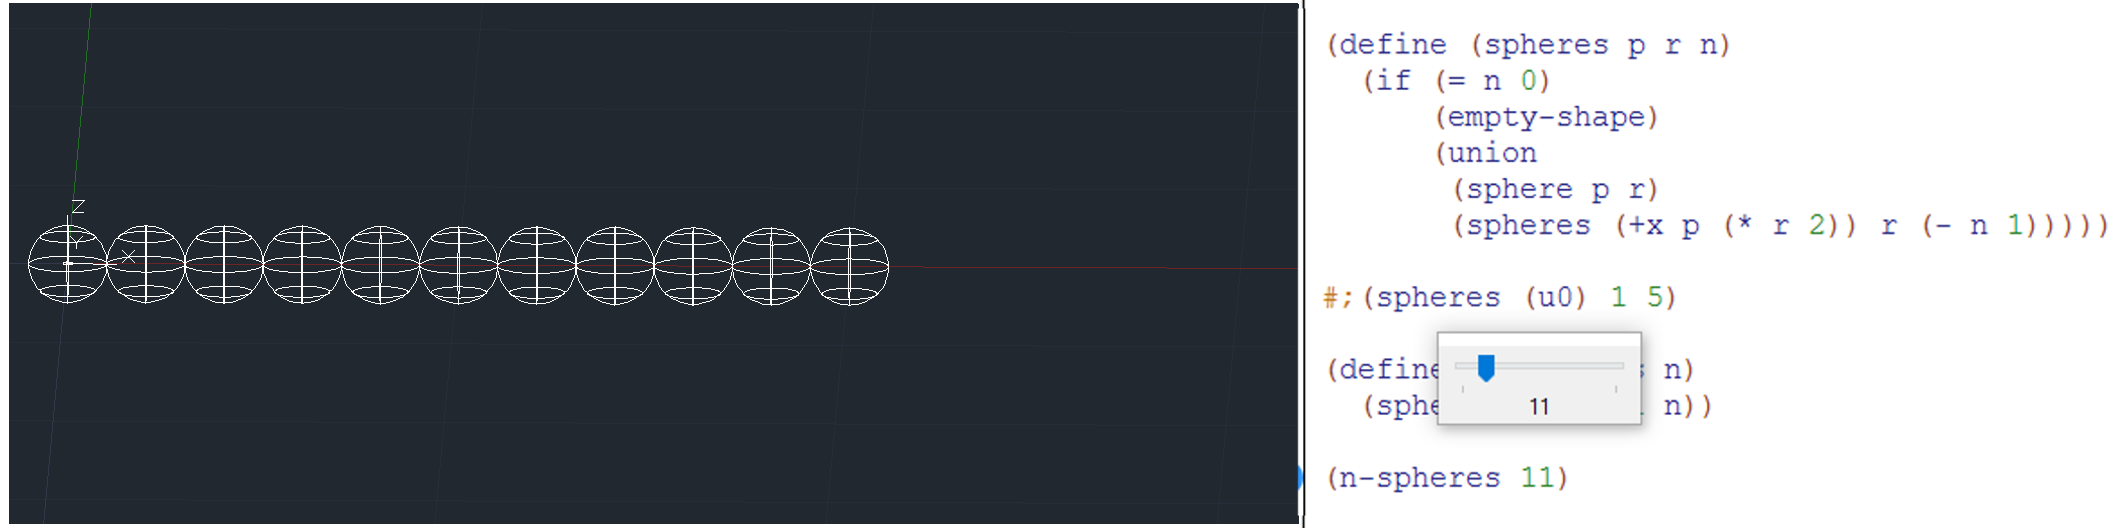
\includegraphics[width=1\textwidth]{images/sliders2}
    \caption{Changing n-spheres input to 11 spheres using a slider.}
  \label{fig:s2}
\end{figure}

\begin{figure}[!h]
  \centering
  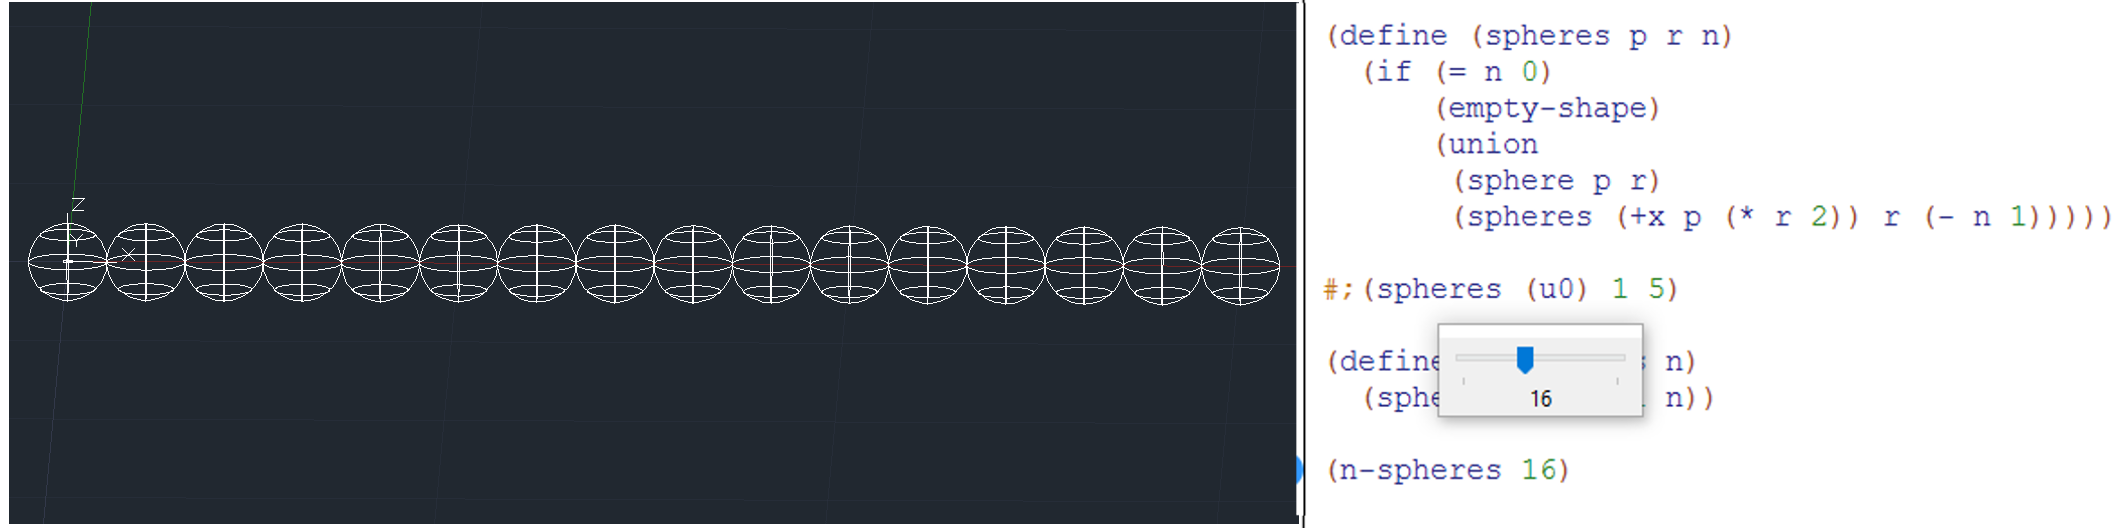
\includegraphics[width=1\textwidth]{images/sliders3}
    \caption{Changing n-spheres input to 16 spheres using a slider.}
  \label{fig:s3}
\end{figure}

Figure~\ref{fig:sturbine1} and Figure~\ref{fig:sturbine2} show the generation of two different shapes of turbines by varying an angle between the fans using a slider.  In this example, the architect triggered the slider widget over an angle denominator. Then, she moved the slider to generate a new geometric model in AutoCAD. 

\begin{figure}[!h]
  \centering
  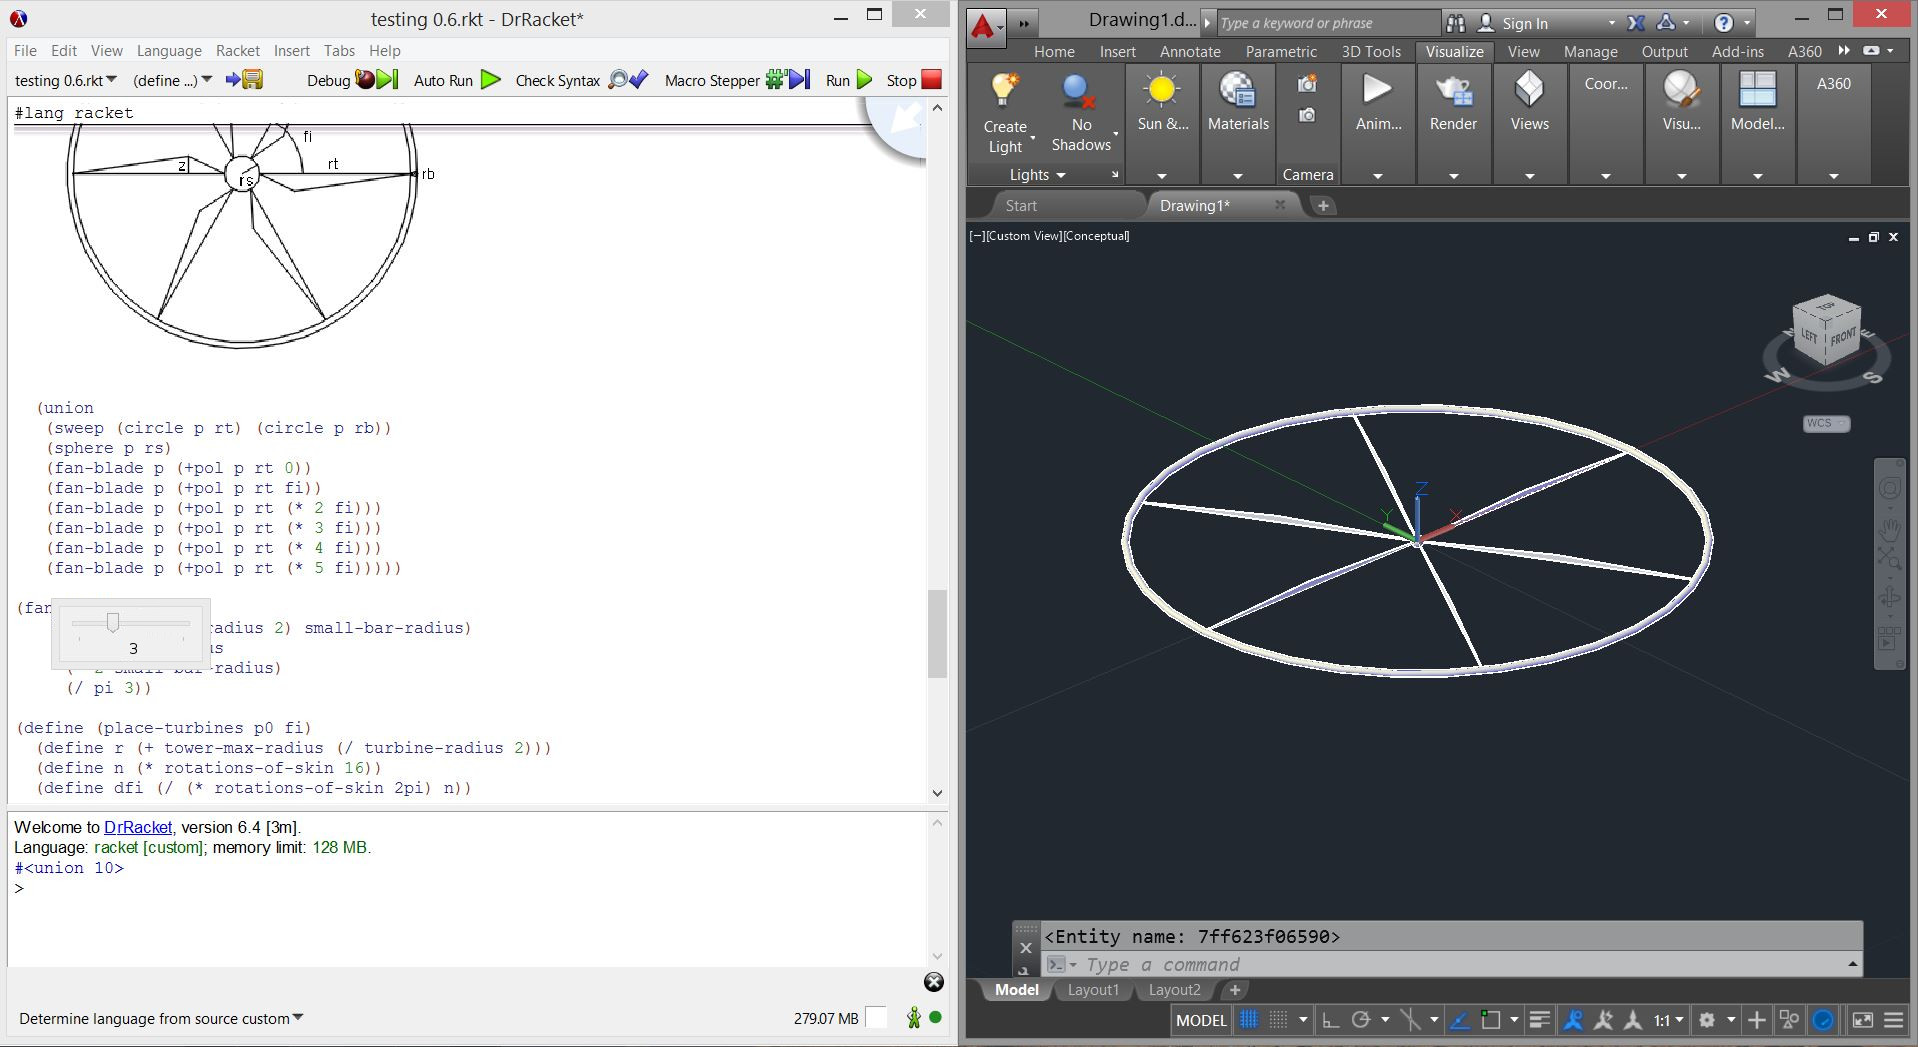
\includegraphics[width=1\textwidth]{images/slider-turbine-1}
    \caption{Using a slider, on the left, to arbitrarily change a number value in the program. The angle denominator has been modified to 3, producing, on the right, the turbine shape with its fans placed over a circumference of $2\pi$ radians.}
  \label{fig:sturbine1}
\end{figure}

\begin{figure}[!h]
  \centering
  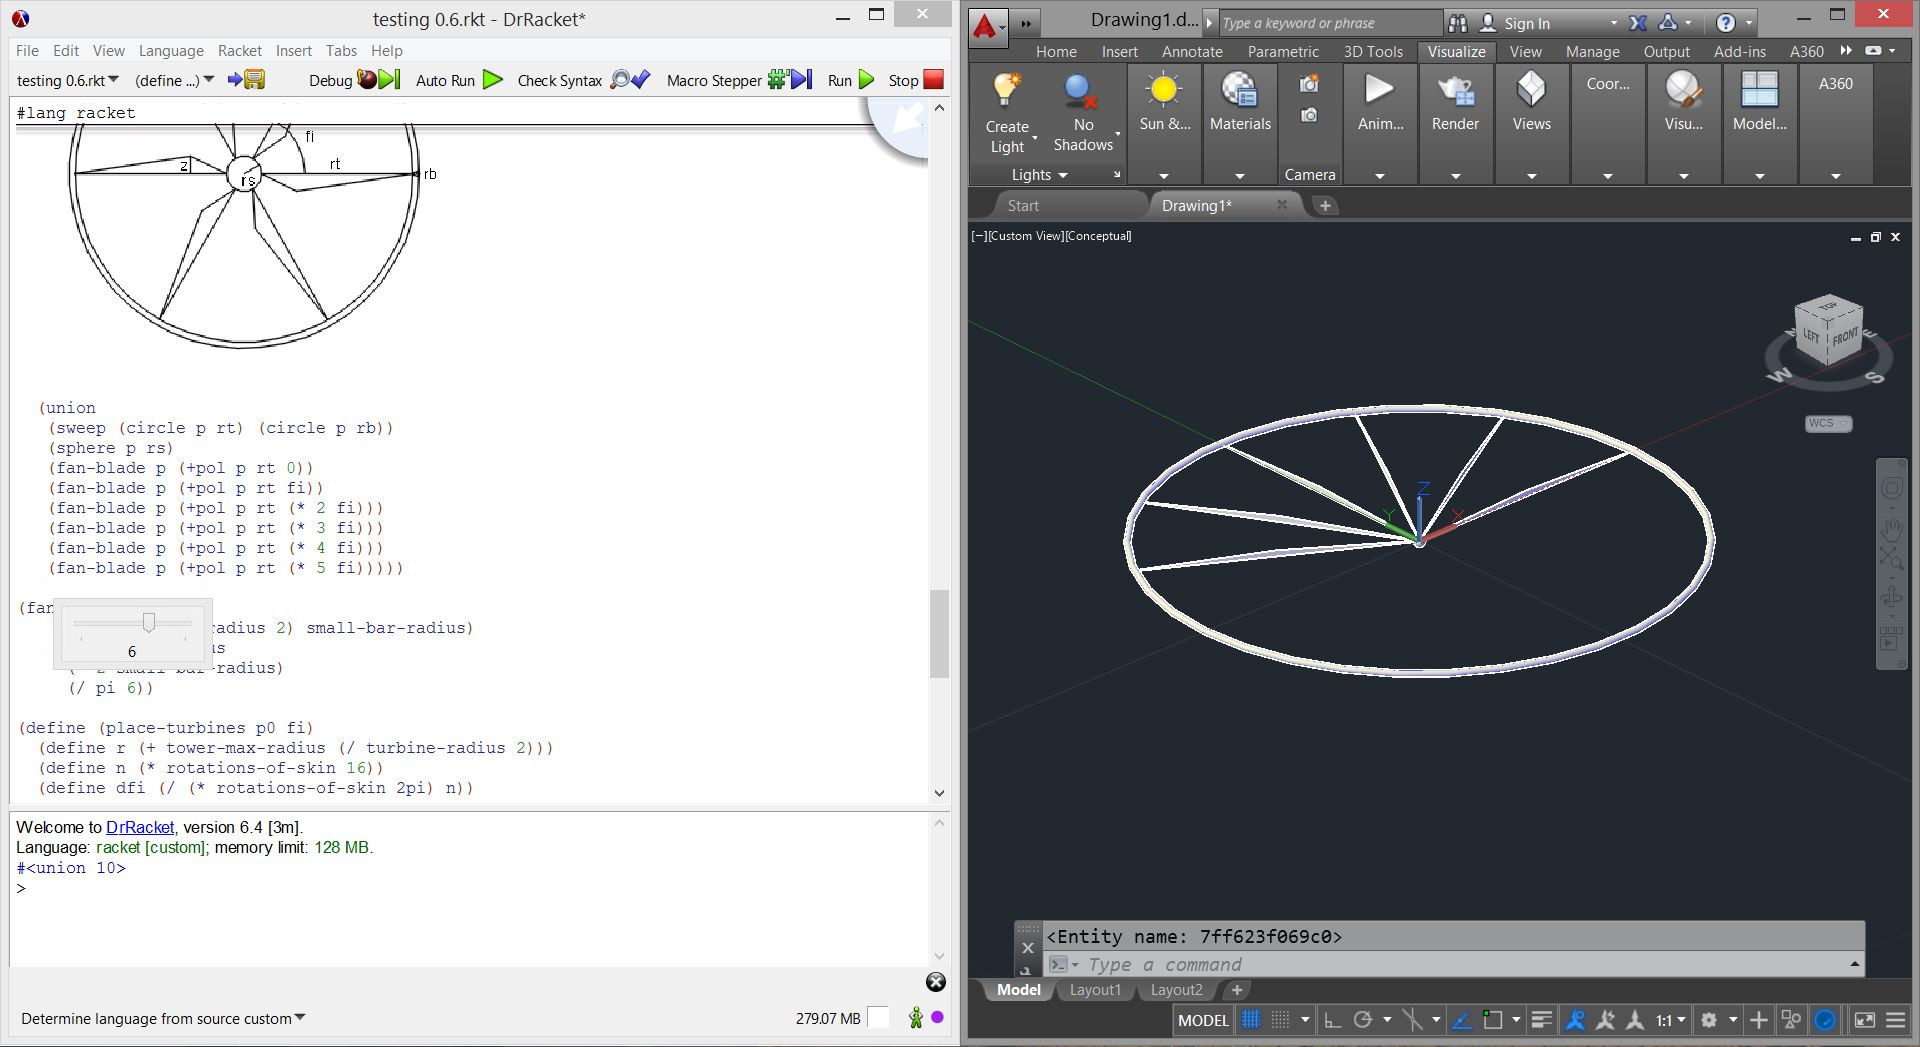
\includegraphics[width=1\textwidth]{images/slider-turbine-2}
    \caption{Using a slider, on the left, to arbitrarily change a number value in the program. The angle denominator has been modified to 6, producing, on the right, the turbine shape with its fans placed over a circumference of $\pi$ radians.}
  \label{fig:sturbine2}
\end{figure}

Figure~\ref{fig:slidermac} shows an example of an architect that unable to use her preferred backend in her operating system, decided to test the AutoRun tool using the factorial function. This example shows DrRacket running on top of MAC OS, supporting the instant feedback mechanism. The slider was used to vary the factorial input, displaying the result in the interactions window. As we can see this tool is independent of the Rosetta tool and, in this example, was applied to a custom user function.

\begin{figure}[!h]
  \centering
  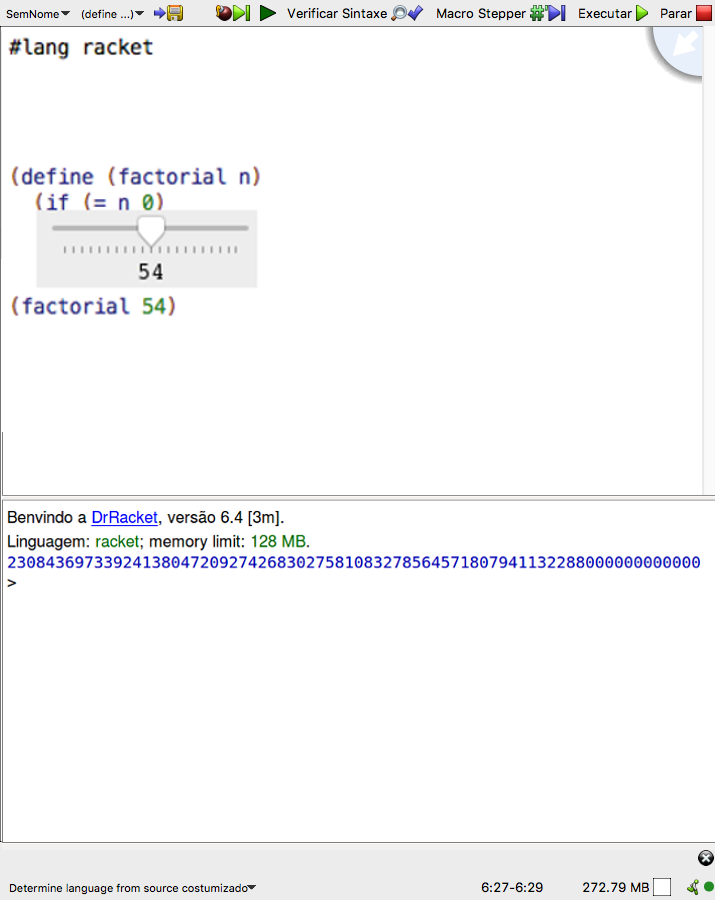
\includegraphics[width=0.6\textwidth]{images/slider-mac}
    \caption{Running factorial function using the slider.}
  \label{fig:slidermac}
\end{figure}


\section{Conclusion}
\label{sec:eval}

The proposed tools, namely the immediate feedback and sketch correlation program tool, were evaluated based on two distinct forms: (1) during the development phase, and (2) after the implementation, as a validation test performed by the target users. In the first stage, I performed a functional analysis, checking if the added features do not interfere with the correct behavior of the programs. After concluding this phase, the tools were ready to be tested by the final users. In the second stage, I tested these features with users and collected some interesting feedback. 

It was an interactive process, as I was receiving the users comments I was fixing the tools. For example, some relevant comments are described as follows:

\begin{itemize}
\item \textit{Sketch-program correlation tool} was reported as a useful tool to document programs, adding a rich source of information for who will use the code. However, some users has trouble to use the fallback mechanism to correct the image pointing arrows. The reported bug was that the key bindings associated with this feature did not work on some operating systems. To fix this problem, the keybindings were changed to a single right click to expand or collapse the images, and a single left click to set its parameters. After this improvement, the reported user experiences were substantially better.

\item On the other hand, \textit{AutoRun} had no issues related to its use; it works correctly on all operating systems, including the slider mechanism. However, a very requested feature was the adaptative slider, which means dynamically changing the slider interval range based on the currently selected value. Unfortunately, as discussed in Chapter~\ref{chapter:evaluation}, this feature is inherently limited by the used DrRacket slider \gls{ui}.
\end{itemize}
